\documentclass[a4paper]{article}

%% Language and font encodings
\usepackage[spanish]{babel}
\usepackage[utf8x]{inputenc}
\usepackage[T1]{fontenc}
\usepackage{listings}

%% Sets page size and margins
\usepackage[a4paper,top=3cm,bottom=2cm,left=3cm,right=3cm,marginparwidth=1.75cm]{geometry}

%% Useful packages
\usepackage{amsmath}
\usepackage{graphicx}
\usepackage[colorinlistoftodos]{todonotes}
\usepackage[colorlinks=true, allcolors=blue]{hyperref}

\title{Practica 3: Teor\'ia de Colas}
\begin{document}
\maketitle

\begin{abstract}
En esta práctica el interés será comparar los tiempos de ejecución de diversos modos de ordenamiento de números ya establecidos, variando la cantidad de núcleos del ordenador utilizados para la misma.
\end{abstract}

\section{Introducci\'on}
La tarea en específico consistirá en saber si un número es primo o no, bien podemos dar una lista de números ya establecida para checar o podemos pedirle que compruebe de un cierto número a otro si lo es. La teoría de Colas entra en nuestra experimentación cuando observamos que para checar si un número en efecto es primo tarda diferente dependiendo si el número es muy grande o muy pequeño, de aquí que lo pudiéramos visualizar como si tuviéramos una cantidad de números por analizar, y varias “máquinas” o líneas para procesarlo, en este caso nuestros núcleos. 

Hasta este punto podríamos suponer que si tengo menos núcleos los tiempos en “línea” serán más grandes, pero veamos si esto ocurre en la práctica,tendremos 3 formas diferentes de checar los números deseados, de manera ascendente, descendente y de forma aleatoria.

\section{Par\'ametros de Trabajo}

Para llevar a cabo la experimentación se realizó en una MacBook Pro la cual cuenta con 4 núcleos disponibles, como es necesario disponer de uno de los núcleos para las ejecuciones, la experimentación la realizaremos desde uno hasta tres núcleos, de igual forma ordenaremos los números con un número de repeticiones fijo, en nuestro caso serán 20 repeticiones, de las cuales se comprobarán números desde mil hasta tres mil.

\section{Modificaciones del código}

Para la primer parte de la tarea lo único que fue necesario incluir fue la automatización para cambiar la cantidad de núcleos utilizados, así como la generación de las gráficas para cada una de las corridas con los núcleos, para esto se agregó lo siguiente al código:

\lstset{language=R, breaklines=true, basicstyle=\footnotesize}

\begin{lstlisting}[frame=single]
for(num in 1: (detectCores()-1)){
registerDoParallel(makeCluster(num))
.
.
.
salida = paste("p3_t", num, ".png", sep="")
png(salida)
boxplot(ot, it, at)
graphics.off()
}
\end{lstlisting}

\section{Resultados}
A continuación presentaremos los gráficos variando la cantidad de núcleos como se especifica de cada uno en el pie del gráfico.

\begin{figure}
\centering
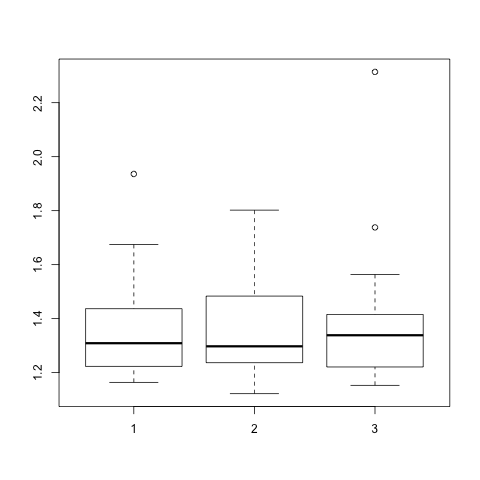
\includegraphics[width=0.7\linewidth]{p3_t1}
\caption[3 Núcleo]{3 Núcleo}
\label{fig:3Núcleos}
\end{figure}

\begin{figure}
\centering
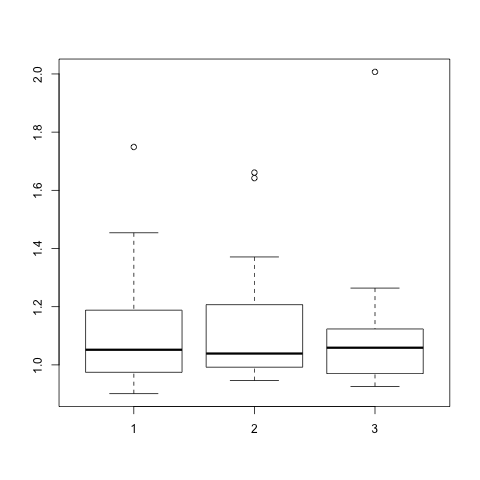
\includegraphics[width=0.7\linewidth]{p3_t2}
\caption[2 Núcleo]{2 Núcleo}
\label{fig:2 Núcleos}
\end{figure}

\begin{figure}
\centering
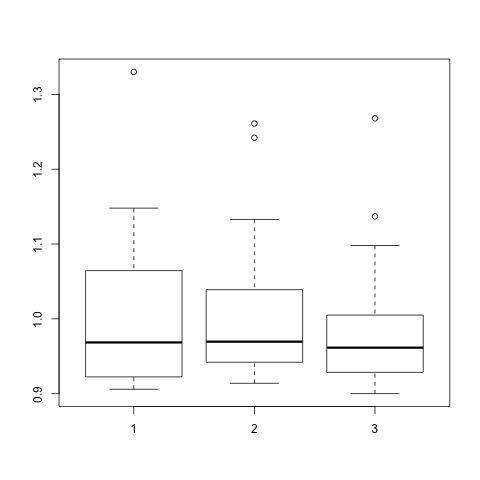
\includegraphics[width=0.7\linewidth]{p3_t3}
\caption[1 Núcleo]{1 Núcleo}
\label{fig:p1 Núcleo}
\end{figure}

\subsection{Interpretación}



\end{document}